\documentclass[12pt]{book} 

\usepackage{amsmath}
\usepackage{graphicx}
\usepackage{import}
\usepackage{amsfonts}
\usepackage{booktabs}

\setlength{\parindent}{0em}  % sets auto indent at new paragraph to none

\newcommand{\incfig}[1]{%
        \import{./figures/}{#1.pdf_tex}
}

\newcommand{\incimg}[2]{%
       \begin{figure}[h]
               \centering
               \includegraphics[scale = #2]{./figures/#1}
       \end{figure}
}

\title{\coursetitle\linebreak\lecturename}
\author{\\Cain Susko\\ 
           \\ \\ \\
      Queen's University 
    \\School of Computing\\} 

%=-=-=-=-=-title-=-=-=-=-=%
\newcommand{\lecturename}{Hash Table Effieciency and Other Types}
\newcommand{\coursetitle}{Data Structures}
%=-=-=-=-=-#####-=-=-=-=-=%

\begin{document}
\begin{titlepage}
        \maketitle
\end{titlepage}


\section*{Hash Table Effieciency}
this effieciency of a hash table os mainly dictated by the complexity of the \texttt{locate} and \texttt{insert} functions.

These complexities depends on the type of hash table (closed v. open), how full the table is, and how many collisions there are in the hash table.

In the worst case, all elements are hashed into the same bucket (list at index of `bucket') as the search time is relative to the number of 
elements in the bucket. In parctice however, this does not happen as hast tables are carefully designed to avoid this.

Witin a hash table, every key $k$ is equally likely to hash to the $m$ buckets.

\paragraph{Open Hash Table Effieiency}
If you have a good hash function, there are $N$ items distrubuted over $M$ buckets. This means that the \textit{load} of the hash table is:
\[ \alpha = \frac{N}{M}\]

A successful search results in the list in the bucket being searched with the average number of comparisons being:
\[S_\alpha = 1 + \frac{N-1}{2M} = 1 + \frac{\alpha}{2}\]
a unsuccessful search will result in an average complexity of 
$\Theta(1+\alpha)$

\paragraph{Closed Hash Table Efficeiency}
within a closed hash table, when it is quite empty, the time complexity is nearly 1. when the hash table is nearly full, the time complexity can be
nearly $O(N)$.

\paragraph{Linear Probing}
the average number of searches during a successful search as a function of the load factor $\alpha$ is:
\incimg{aAvg}{0.2}

there is a tradeoff as the larger the hash table, the faster it is. however that requires more memory, less memeory means slower hash table. in order to 
resolve both these issues we can implement rehasing

\section*{Re Hashing}
for seperate chaining we can rehash the function $h_1(x) = m\mod 5$ to be $h_2(x) = m\mod 11$
\incimg{rehash}{0.5}

\paragraph{Quadratic Probing}
Additionally, a draw on time is when linear probing checks many already-full buckets. To avoid this, we can use something
called Quadratic Probing.
\incimg{quad}{0.5}

Note: $c_2 \neq 0$
\pagebreak

\section*{Examples}
\begin{figure}[h]
        \centering
        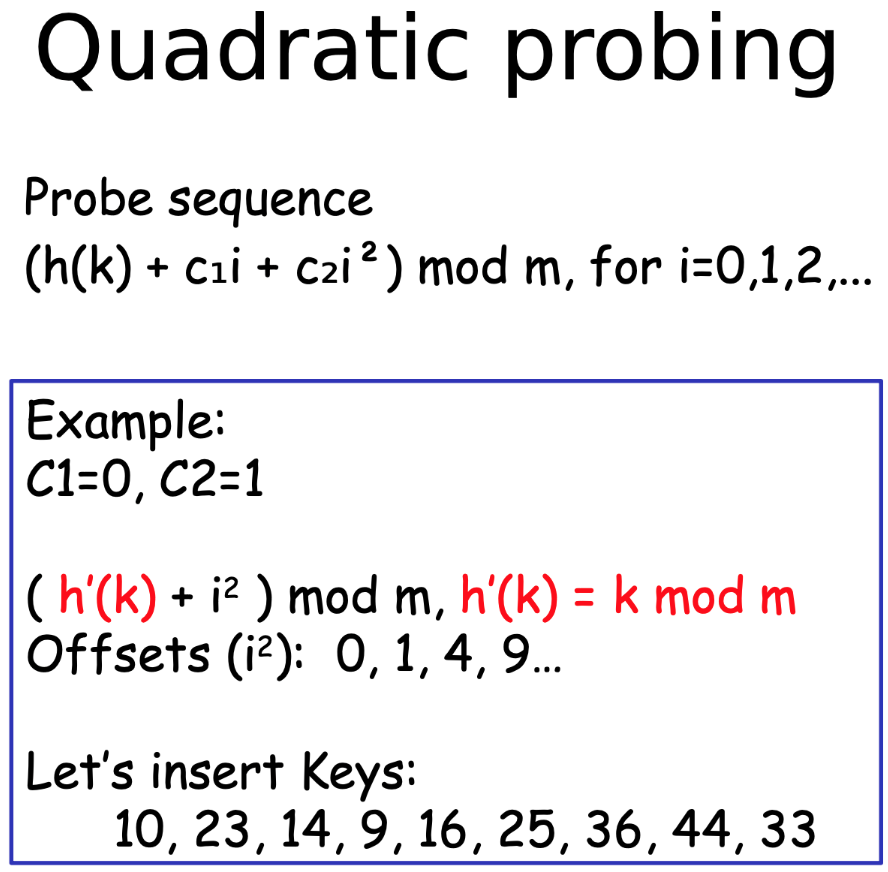
\includegraphics[scale=0.3]{./figures/ex1}
        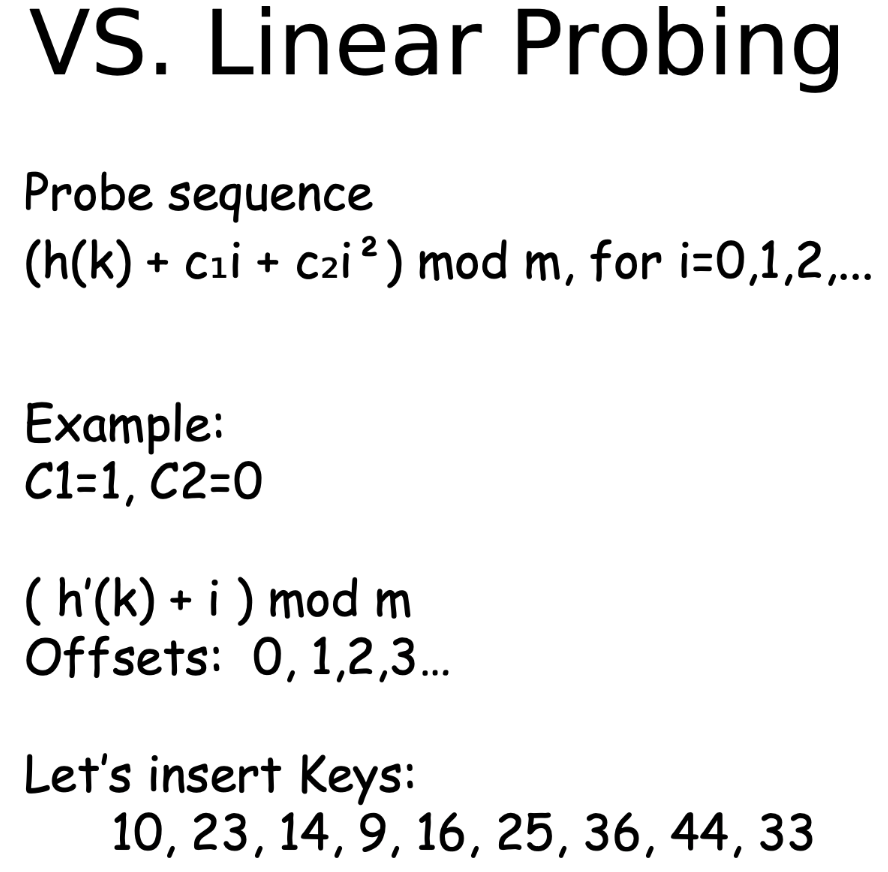
\includegraphics[scale=0.3]{./figures/ex2}
\end{figure}

An implementation of quadratic probing would be as follows:
\incimg{code}{0.5}

\paragraph{Problems with Quadratic Probing}
There are some problems with Qudratic Probing however, mainly it is that the entire probing sequece is determined by the initial probe.
A much larger problem with quadratic probing is that, if given
\incimg{probe}{0.5}
the probe sequence for $h'(k) = 0$ is:
\[0,2,6,0,8,6,6,0,8,6,...\]
which will \textit{never} caontain any odd numbers, so our table couls only be half full but the hash function would say it is full...

In order to avoid this, we must control the load factor and table size such that:
\[\alpha \leq 0.5\]
\[prime(N) = \texttt{true}\]

where $\alpha$ is the load factor and $N$ is the number of items contained in the hash table.
Another way to avoid this problem altogether is by using double hashing instead of quadratic probing.

\section*{Double Hashing}
The idea of double hasing is to using a second hash function to spread out the search for an empty slot. double hashing is one of the most efficient
collosion avoidance methodes to use. An Example equation is:
\[h(i, k) = (h_1(k) + i*h_2(k)) \mod m\]

due to the fact that $h_2(k)$ and $m$ are relatively prime for all $k$, each probing sequence \textbf{contains all addresses!}
\incimg{doublehash}{0.4}

within double factoring, the load factor for the successful and unsuccessful search are:
\[\frac{1}{1-\lambda}\;\;\;\;\;\;\;\;\frac{1}{\lambda}\ln\left(\frac{1}{1-\lambda}\right)\]
\end{document}

